\textbf{Question N2:}

\uline{General Explanation of the plots:}

blue background - goal classifier

green and red points- example nodes labeled 1 and 0 respectively.

x Markers - test examples we discussing.

red lines- goal classifier returns 0

blue lines- goal classifier returns 1

\textbf{(a)}

$D=\{<(0,1),1>,<(0,-1),0>\}$

classifier $F_{true}=1\ if\ v_{2}>0$

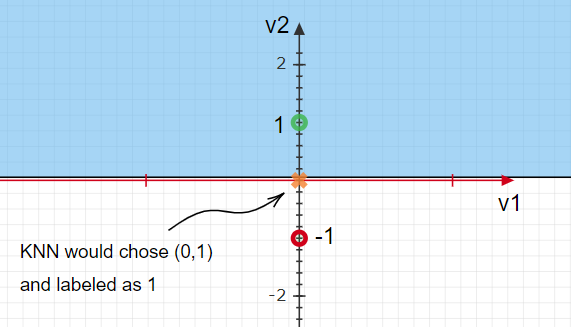
\includegraphics[bb = 0 0 200 100, draft, type=eps]{pic_Q2_HW3/a.png}

ID3: $v_{1}$ feature isn't informative and by using $v_{2}$ we reach
the leaves. ID3 will check if $v_{2}$>0 (zero is the avg. of $v_{2}$)
and we will find the goal classifier.

KNN:

for testing point $x_{q}=(0,0)$: $d(x_{q},(0,1))=d(x_{q},(0,-1))$
thus we choose the node with higher $v_{2}$ and returning its label,
i.e. $KNN(x_{q})=1$ and that is wrong.

We found that $\nexists x_{q}:\ KNN(x_{q})\neq F_{true}$ .

\textbf{Thus ID3 Right and KNN not always.}

\_\_\_

\textbf{(b)}

$D=\{<(1,-1),1>,<(-1,1),0>\}$

classifier: $F_{true}=\begin{array}{c}
1\;v1\geq v2\\
0\;v1<v2
\end{array}$

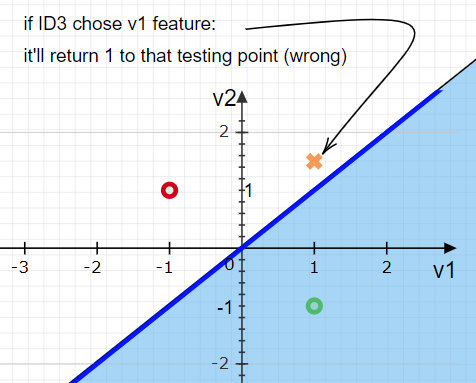
\includegraphics[bb = 0 0 200 100, draft, type=eps]{pic_Q2_HW3/b.png}

The ID3 will use only one feature cause after one division it riches
a leaf e.g. taking $v1>0\ or\ v2>0$ and this is clearly bad. (see
image)

KNN will be right in every situation. if $x_{q}$features are equal
$v_{1}=v_{2}$ , the distances to both training nodes are equal and
it will take the positive nodes $<(1,-1),1>$ because of higher $v_{1}$
which is consistent with the true classifier. Else $x_{q}:v_{1}\neq v_{2}$
it will classify right by computing the distances to the nearest example
node.

Thus \textbf{KNN always Right and ID3 not always right}

\_\_\_\_

\textbf{(c) }

choose K=1

$D=\{<(1,-1),1>,<(-1,1),0>\}$

classifier: $F_{true}=\begin{array}{c}
1\;v1>v2\\
0\;v1\leq v2
\end{array}$

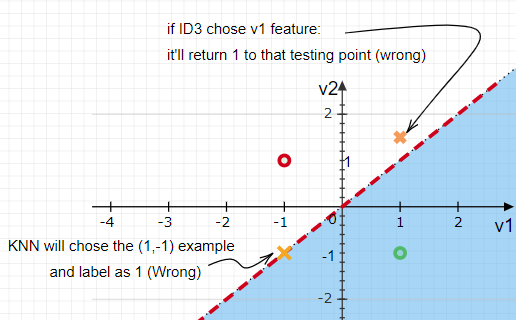
\includegraphics[bb = 0 0 200 100, draft, type=eps]{pic_Q2_HW3/c.png}

The ID3 will use only one feature cause after one division it riches
a leaf e.g. taking $v1>0\ or\ v2>0$ and this is clearly bad. (see
image)

KNN will be wrong at points whose $v_{1}=v_{2}$: the distances to
both training nodes are equal and it will take the positive nodes
$<(1,-1),1>$ because of higher $v_{1}$ and return True (1).

However the true classifier will label it as False (0).

Thus \textbf{ID3 and KNN not always right .}

\_\_\_\_\_\_\_\_\_\_

\textbf{(d)}

K=1:

$D=\{<(0,1),1>,<(0,-1),0>\}$

classifier $F_{true}=1\ if\ v_{2}\geq0$

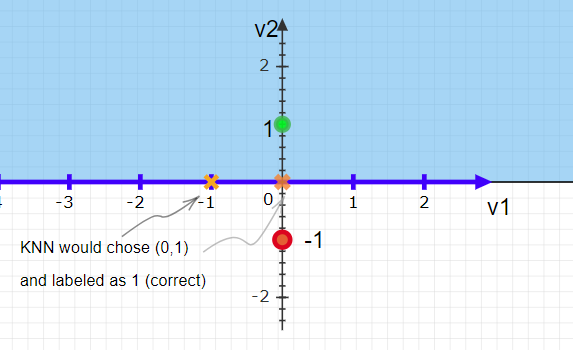
\includegraphics[bb = 0 0 200 100, draft, type=eps]{pic_Q2_HW3/d.png}

ID3: $v_{1}$ feature isn't informative and by using $v_{2}$ we can
get to the leaves. ID3 will check if $v_{2}$>0 and we will get the
goal classifier.

KNN:

if $x_{q}:v2=0$, the distance to the examples are equal and the label
will be taken from the higher $v_{2}$ example and return 1 (Right).

else ($v_{2}\neq0)$ the KNN is working good. for $v_{2}>0$ the nearest
example is (0,1) and the label is 1 and for $v_{1}<0$ the nearest
example is (0,-1) and the label is 0, thus in both cases it is consistent
with classifier).

Thus \textbf{KNN and ID3 are always right}
